\documentclass[13pt]{beamer}

%% Packages

\usepackage{mathtools, amsthm}
% \usepackage{tikz}
% \usetikzlibrary{positioning}
% \usepackage{csquotes}
% \usepackage{hyperref}

%% Environments

\theoremstyle{plain} % default
\newtheorem{teo}{Teorema}[section]
\newtheorem*{teo*}{Teorema}
\newtheorem{lem}{Lema}[section]
\newtheorem{prop}{Proposição}[section]
\newtheorem{cor}[teo]{Corolário}
\newtheorem*{axiom}{Axioma}

\newtheorem*{TAU}{Teorema da Aproximação Universal}
\newtheorem*{Riesz}{Teorema da Representação de Riesz}

\theoremstyle{definition}
\newtheorem{defn}{Definição}[section]
\newtheorem{conj}{Conjectura}[section]
\newtheorem{exmp}{Exemplo}[section]
\newtheorem{rem}{Observação}[section]
\newtheorem*{rem*}{Observação}

\theoremstyle{remark}
\newtheorem*{note}{Nota}
\newtheorem{case}{Caso}


% Macros

\renewcommand{\vec}[1]{\mathbf{#1}}
\renewcommand{\Re}{\text{Re}}

\newcommand{\K}{\mathbb{K}}
\newcommand{\I}{\mathbb{I}}

\DeclarePairedDelimiter{\dotprod}{\langle}{\rangle}

\DeclareMathOperator{\rk}{rk}
\DeclareMathOperator{\intt}{int}
\DeclareMathOperator{\diam}{diam}
\DeclareMathOperator{\rref}{rref}
\DeclareMathOperator{\vspan}{span}
\DeclareMathOperator{\proj}{proj}
\DeclareMathOperator{\lin}{Lin}
\DeclareMathOperator{\supp}{supp}

\newcommand{\func}[3]{#1 : #2 \rightarrow #3}
\newcommand{\R}{\mathbb{R}}
\newcommand{\Z}{\mathbb{Z}}
\newcommand{\N}{\mathbb{N}}
\newcommand{\Q}{\mathbb{Q}}
\newcommand{\rr}{R_{r}}
\newcommand{\tq}{ : }
\newcommand{\mdc}{\text{mdc}}
\newcommand{\mmc}{\text{mmc}}
\newcommand{\defeq}{\vcentcolon=}
\newcommand{\comp}{\mathscr{C}}


%% Upper and Lower Integrals
\newcommand{\loint}[4]{
    \lefteqn{\int_{ #1 }^{ #2 } #3}\lefteqn{\hspace{0.0ex}\rule[-2.25ex]{1.1ex}{.05ex}} \phantom{\int_{ #1 }^{ #2 } #3}\mathrm{d}#4
}
\newcommand{\upint}[4]{
    \lefteqn{\int_{ #1 }^{ #2 } #3 \ }\lefteqn{\hspace{1.2ex}\rule[ 3.35ex]{1.1ex}{.05ex}} \phantom{\int_{ #1 }^{ #2 } #3 \ }\mathrm{d}#4
}

\DeclarePairedDelimiter\ceil{\lceil}{\rceil}
\DeclarePairedDelimiter\floor{\lfloor}{\rfloor}
\DeclarePairedDelimiter\abs{\lvert}{\rvert}%
\DeclarePairedDelimiter\norm{\lVert}{\rVert}%
\DeclareMathOperator{\sen}{sen}

% Swap the definition of \abs* and \norm*, so that \abs
% and \norm resizes the size of the brackets, and the 
% starred version does not.

\makeatletter
\let\oldabs\abs
\def\abs{\@ifstar{\oldabs}{\oldabs*}}
%
\let\oldnorm\norm
\def\norm{\@ifstar{\oldnorm}{\oldnorm*}}
\makeatother

\newcommand{\transpose}{\mathsf{T}}

\usepackage{global-macros}
\usepackage{siunitx}

\begin{comment}
\end{comment}

\title[Modelagem do Tratamento para HIV]{Modelagem Matemática do Tratamento para Infecção por HIV}
\author[C. Lins, J. Martins]{Caio Lins \and Juliane Martins}
\institute[EMAp]{FGV - EMAp}
\date[EMAp 2021]{Novembro 2021}
\logo{
\includegraphics[height=0.8cm]{../figuras/fgv_logo.png}}


\begin{document}

\maketitle

\begin{frame}{A Infecção por HIV}
    \begin{itemize}
        \item<1-> \textit{Human Immunodeficiency Virus} -- uma das principais causas de mortalidade do mundo.

        \item<2-> Vírus provoca a morte de células T-CD4+, que são parte vital do sistema imunológico.

        \item<3-> O tratamento para infecção por HIV é denominado ART -- \textit{Antiretroviral Drug Therapy}.

    \end{itemize}
\end{frame}

\begin{frame}{Tratamento com Combinação de Drogas}
    Exploraremos o efeito do tratamento realizado com uma combinação de dois tipos de drogas:
    \begin{itemize}
        \item<2-> Inibidor de transcriptase reversa: atua impedindo a infecção de novas células pelo HIV.
        \item<3-> Inibidor de protease: atua prejudicando a formação de novas partículas virais dentro de células já infectadas.
    \end{itemize}
\end{frame}

\begin{frame}{Modelo para a doença \textbf{sem tratamento}}

%     \begin{tikzpicture}[auto, >=latex']
%         \node [block, pin={[pin edge={arrow,<-}] above left: \( S ( t ) \)}] (s) {\( T \)};
%         \node [block, right = 2.5cm of s] (p) {\( T_{ s } \)};
%         \node [block, above right = 0.25cm and 1cm of p] (a) {Infected, \\ Asymptomatic \\ $A$};
%         \node [block, below right = 0.25cm and 1cm of p] (i) {Infected, \\ Sympomatic \\ $I$};
%         \node [block, right = 1cm of a] (r) {Recovered, \\ Immune \\ $R$};
%         \node [block, right = 1cm of i] (d) {Dead \\ $D$};
% 
%         \draw [arrow] (s) -- node [above] {$b_PPS+b_AAS$} node [below] {$+b_IIS$} (p);
%         \draw [arrow] (p.north) |- ++(0cm,+1.5cm) -- node [above] {$fg_PP$} (a.west);
%         \draw [arrow] (p.south) |- ++(0cm,-1.5cm) -- node [below] {$(1-f)g_P P$} (i.west);
%         \draw [arrow] (a) -- node [above] {$g_A A$} (r);
%         \draw [arrow] (i) -- node [below] {$d g_I I$} (d);
%         \draw [arrow] (i) -- node [above, xshift = 1cm,yshift = -0.2cm] {$(1-d) g_I I$} (r);
%         \draw [arrow] (r.north) |- ++(0cm,+1.0cm) -- node [above, pos = 0.75mm] {$wR$} ++(-3cm,0cm) -| (s);
% 
%     \end{tikzpicture}

    Temos três populações:
    \begin{itemize}
        \item \( T ( t ) \): Células T saudáveis
        \item \( T_{ s } ( t ) \): Células T infectadas
        \item \( V_{ s } ( t ) \): Partículas virais suscetíveis
    \end{itemize}

    Todas são medidas em indivíduos por \( \unit{mm^{ 3 }} \) no plasma sanguíneo.
    
\end{frame}

\begin{frame}{Modelo para a doença \textbf{sem tratamento}}{Equação para \( T ( t ) \)}
    \begin{equation*}
        \dot{ T } ( t ) = S ( t ) - \mu_{ T } T ( t ) + p T ( t ) \frac{ V_{ s } ( t ) }{ C + V_{ s } ( t ) } - k_{ s } V_{ s } ( t ) T ( t ) \label{Tponto_S}
    \end{equation*}
    \begin{itemize}
        \item<2-> \( S ( t ) \): Produção natural de células \( T \) pelo corpo

            \begin{equation*}
                S ( t ) = 10 - 7 \frac{ V ( t ) }{ B_{ s } + V ( t ) }
            .\end{equation*}

        \item<3-> \( \mu_{ T } T ( t ) \): Morte natural de células \( T \).
        \item<4-> \( p T ( t ) \frac{ V_{ s } ( t ) }{ C + V_{ s } ( t ) } \): Multiplicação de células T devido à resposta imune.
        \item<5-> \( k_{ s } V_{ s } ( t ) T ( t ) \): Infecção de células T pelo HIV.
    \end{itemize}
\end{frame}

\begin{frame}{Modelo para a doença \textbf{sem tratamento}}{Equação para \( T_{ s } ( t ) \)}
    \begin{equation*}
        \dot{T_{ s }} ( t ) = k_{ s } V_{ s } ( t ) T ( t ) - \mu_{ T_{ i } } T_{ s } ( t ) - p_{ i } T_{ s } ( t ) \frac{ V_{ s } ( t ) }{ C_{ i } + V_{ s } ( t ) } \label{Tsponto_S}
    \end{equation*}
    \begin{itemize}
        \item<2-> \( k_{ s } V_{ s } ( t ) T ( t ) \): Infecção de células T pelo HIV.
        \item<3-> \( \mu_{ T_{ i } } T_{ s } ( t ) \): Mortalidade de células T infectadas.
        \item<4-> \( p_{ i } T_{ s } ( t ) \frac{ V_{ s } ( t ) }{ C_{ i } + V_{ s } ( t ) } \): Células infectadas que explodem pelo excesso de partículas virais invasoras.
    \end{itemize}
\end{frame}

\begin{frame}{Modelo para a doença \textbf{sem tratamento}}{Equação para \( V_{ s } ( t ) \)}
    \begin{equation*}
        \dot{V_{ s }} ( t ) = N p_{ i } T_{ s } ( t ) \frac{ V_{ s } ( t ) }{ C_{ i } + V_{ s } ( t ) } - k_{ \nu } T ( t ) V_{ s } ( t ) + G_{ s } \frac{ V_{ s } ( t ) }{ B + V_{ s } ( t ) } \label{Vsponto_S}
    \end{equation*}
    \begin{itemize}
        \item<2-> \( N p_{ i } T_{ s } ( t ) \frac{ V_{ s } ( t ) }{ C_{ i } + V_{ s } ( t ) } \): Partículas virais liberadas pela explosão de células T infectadas.
        \item<3-> \( k_{ \nu } T ( t ) V_{ s } ( t ) \): Morte de partículas virais pela resposta imune.
        \item<4-> \( G_{ s } \frac{ V_{ s } ( t ) }{ B + V_{ s } ( t ) } \): Fonte viral externa ao sangue.
    \end{itemize}
    \visible<5-> {O parâmetro \( G_{ s } \) será o principal fator determinante para o curso geral da infecção.}
\end{frame}

\begin{frame}{Simulações da infecção \textbf{sem tratamento}}
    \begin{figure}[htb]
        Infecção com \( G_{ s } = 80 \)
        \begin{center}
            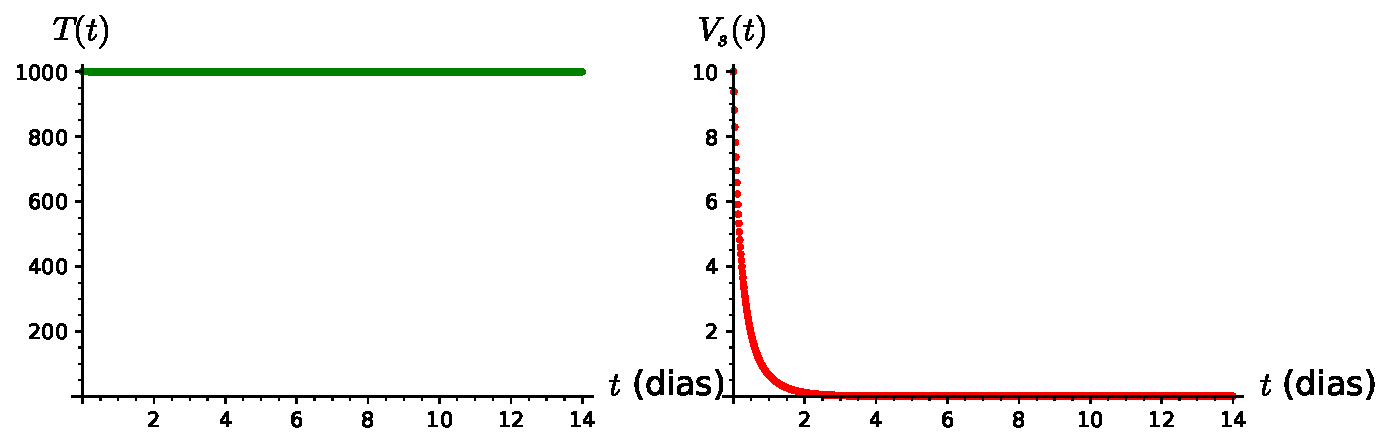
\includegraphics[width=1\textwidth]{../figuras/cenario_1.pdf}
        \end{center}
    \end{figure}
\end{frame}

\begin{frame}{Simulações da infecção \textbf{sem tratamento}}
    \begin{figure}[htb]
        Infecção com \( G_{ s } = 180 \)
        \begin{center}
            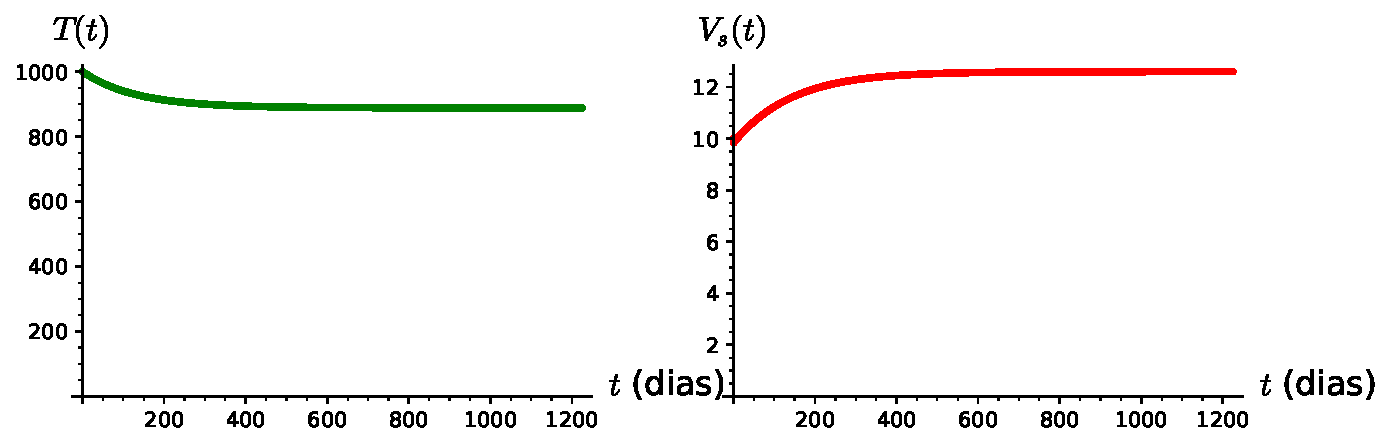
\includegraphics[width=\textwidth]{../figuras/cenario_2.pdf}
        \end{center}
    \end{figure}
\end{frame}

\begin{frame}{Simulações da infecção \textbf{sem tratamento}}
    \begin{figure}[htb]
        Infecção com \( G_{ s } = 330 \)
        \begin{center}
            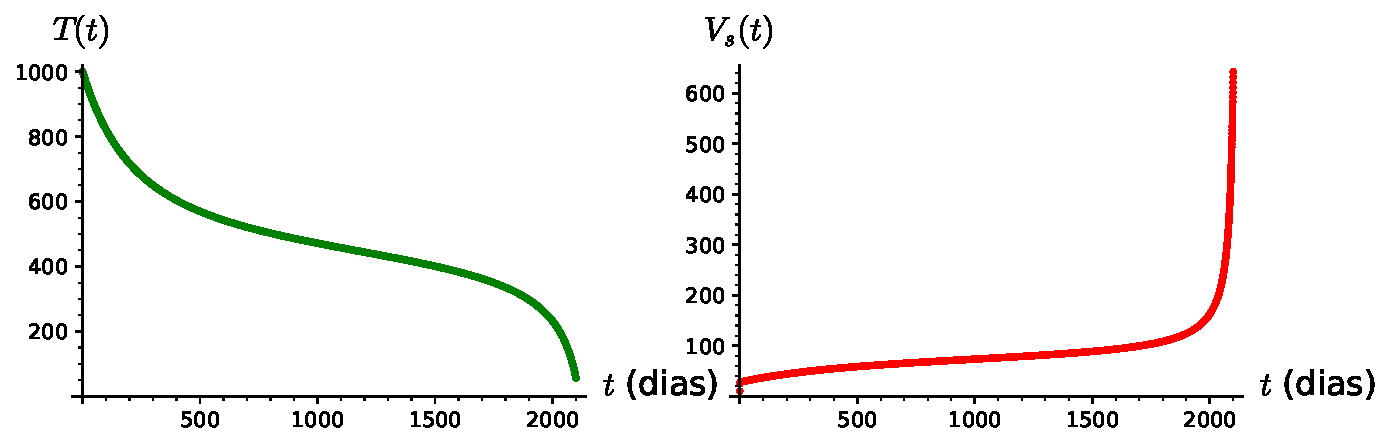
\includegraphics[width=\textwidth]{../figuras/cenario_3.pdf}
        \end{center}
    \end{figure}
\end{frame}

\begin{frame}{Modelo para a doença \textbf{com tratamento}}
    \begin{itemize}
        \item<1-> Simular a infecção sem tratamento até um tempo \( t_{ 0 } \).
        \item<2-> Utilizar os valores de \( T ( t_{ 0 } ), T_{ s } ( t_{ 0 } ) \) e \( V_{ s } ( t_{ 0 } ) \) como valores iniciais para o modelo com tratamento.
        \item<3-> Em um tempo \( t_{ r } > t_{ 0 } \), surge uma variante do vírus resistente ao tratamento.
    \end{itemize}
\end{frame}

\begin{frame}{Modelo para a doença \textbf{com tratamento}}
    Populações novas:
    \begin{itemize}
        \item<1-> \( V_{ r } ( t ) \): Vírus resistente ao tratamento.
        \item<2-> \( T_{ r } ( t ) \): Células T infectadas pelo vírus resistente.
    \end{itemize}
    \visible<3->{Definimos \( V ( t ) \defeq V_{ s } ( t ) + V_{ r } ( t ) \) como a população viral total.}
\end{frame}

\begin{frame}{Modelo para a doença \textbf{com tratamento}}{Equações}
    \begin{align*}
        \dot{T}( t ) &= S_{ 0 } ( t ) - \mu_{ T } T ( t ) + p T ( t ) \frac{ V ( t ) }{ C + V ( t ) } \\
                     &\qquad - ( \mu k_{ s } V_{ s } ( t ) + k_{ r } V_{ r } ( t ) ) T ( t ) \\
        \dot{T_{ s }} ( t ) &= \mu k_{ s } V_{ s } ( t ) T ( t ) - \mu_{ T_{ i } } T_{ s } ( t ) - p_{ i } T_{ s } ( t ) \frac{ V ( t ) }{ C_{ i } + V ( t ) } \\
        \dot{ T_{ r } } ( t ) &= k_{ r } V_{ r } ( t ) T ( t ) - \mu_{ T_{ i } } T_{ r } ( t ) - p_{ i } T_{ r } ( t ) \frac{ V ( t ) }{ C_{ i } + V ( t ) }  \\
    \end{align*}
\end{frame}

\begin{frame}{Modelo para a doença \textbf{com tratamento}}{Equações}
    \begin{align*}
        \dot{V_{ s } } ( t ) &= \rho q ( t ) N p_{ i } T_{ s } ( t ) \frac{ V ( t ) }{ C_{ i } + V ( t ) } + ( 1 - q ( t ) ) N p_{ i } T_{ r } ( t ) \frac{ V ( t ) }{ C_{ i } + V ( t ) } \\
                             &\qquad - k_{ \nu } T_{ t } V_{ s } ( t ) + \eta G_{ s } \frac{ V_{ s } ( t ) }{ B + V ( t ) } \\
        \dot{ V_{ r }} ( t ) &= q ( t ) N p_{ i } T_{ r } ( t ) \frac{ V ( t ) }{ C_{ i } + V ( t ) } + ( 1 - q ( t ) ) N p_{ i } T_{ s } ( t ) \frac{ V ( t ) }{ C_{ i } + V ( t ) } \\
                             &\qquad - k_{ \nu } T ( t ) V_{ r } ( t ) + G_{ r } \frac{ V_{ r } ( t ) }{ B + V ( t ) }
    .\end{align*}
\end{frame}

\begin{frame}{Modelo para a doença \textbf{com tratamento}}{Ideia}
    \begin{itemize}
        \item<1-> Influência do tratamento no vírus \textbf{suscetível}:
            \begin{itemize}
                \item<2-> Termos que representam infecção de células T saudáveis são multiplicados por uma constante \( \mu < 1 \) (inibidor de transcriptase reversa)
                \item<3-> Termo que representa ganho de vírus pela explosão de células T contaminadas é multiplicado por uma constante \( \rho < 1 \) (inibidor de protease).
                \item<4-> Termo que representa ganho de vírus vindo de fora do sangue é multiplicado por uma constante \( \eta < 1 \).
            \end{itemize}
        \item<5-> A partir de \( t_{ r } \), uma proporção \( q \in (0, 1) \) dos vírus gerados sofre uma mutação e passa a ser resistente ao tratamento (modificações acima não se aplicam).
    \end{itemize}
\end{frame}

\begin{frame}{Modelo para a doença \textbf{com tratamento}}{Simulações}
    \begin{itemize}
        \item<1-> Os gráficos representam a evolução das populações a partir do início do tratamento.
        \item<2-> O tratamento foi iniciado quando a população \( T ( t ) \) atingiu uma marca pré-determinada.
        \item<3-> Tomamos \( t_{ r } \) como \( 30 \) semanas após o início do tratamento.
    \end{itemize}
\end{frame}

\begin{frame}{Modelo para a doença \textbf{com tratamento}}{Simulações}
    \begin{figure}
        Tratamento iniciado quando \( T ( t ) = 200 \)
        \begin{center}
            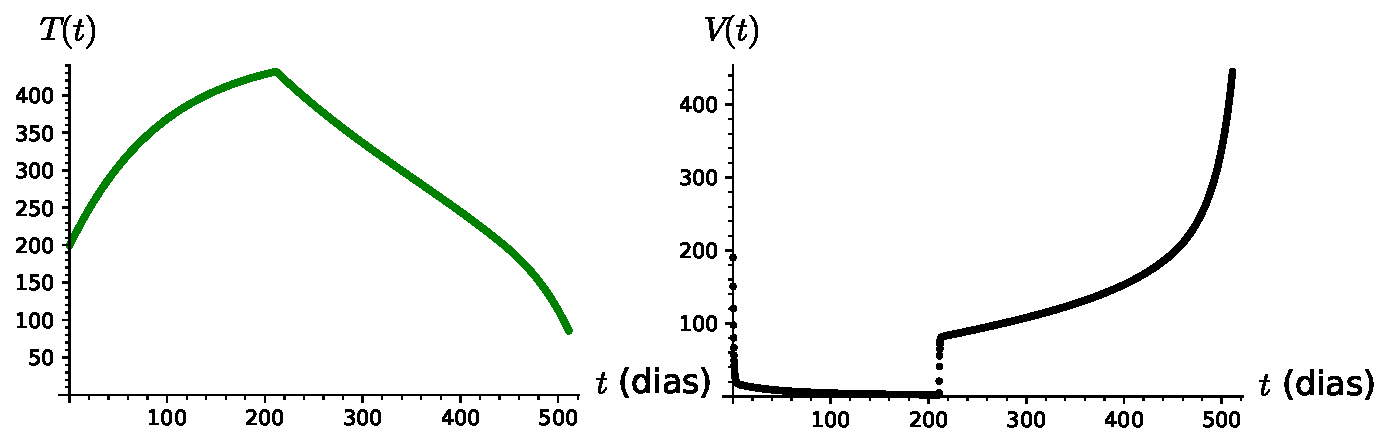
\includegraphics[width=\textwidth]{../figuras/start_treatment_at_T_200.pdf}
        \end{center}
    \end{figure}
\end{frame}

\begin{frame}{Modelo para a doença \textbf{com tratamento}}{Simulações}
    \begin{figure}
        Tratamento iniciado quando \( T ( t ) = 300 \)
        \begin{center}
            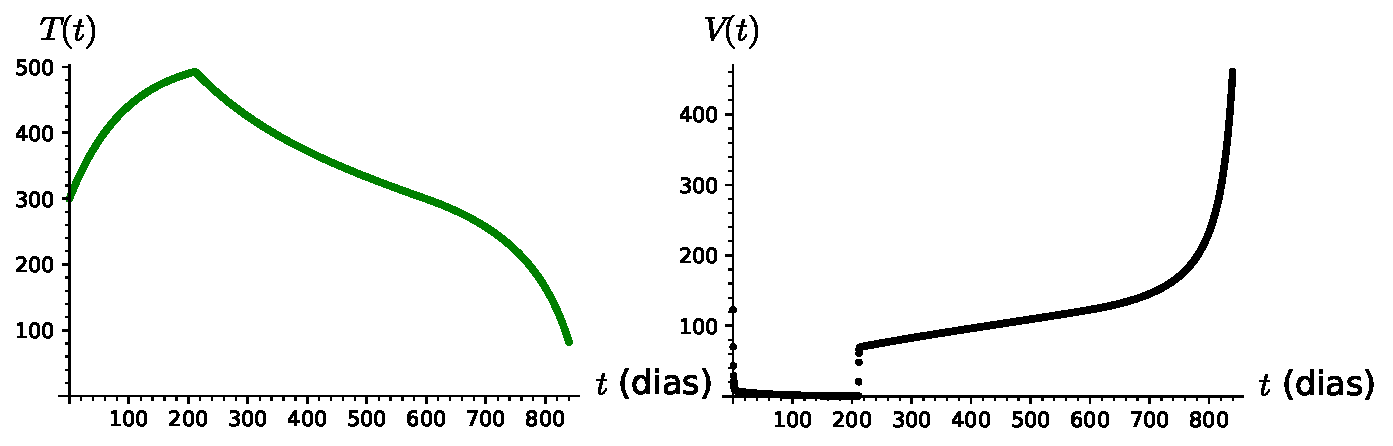
\includegraphics[width=\textwidth]{../figuras/start_treatment_at_T_300.pdf}
        \end{center}
    \end{figure}
\end{frame}

\end{document}
